\subsection{Le calorimètre électromagnétique ou ECAL}\label{chapter-LHC-section-CMS-subsec-ECAL}
%\cite{cms_paper,CERN-LHCC-97-033,CMS-CR-1999-006,CMS-EGM-11-001,CMS-CR-2014-410,CMS-DP-2016-031,CMS-CR-2018-162,CMS-DP-2019-005,CMS-DP-2020-021}
Le calorimètre électromagnétique (ECAL)~\cite{cms_paper,CERN-LHCC-97-033,CMS-EGM-11-001,CMS-DP-2019-005,CMS-DP-2020-021} permet de mesurer l'énergie des électrons et des photons par un processus destructif.
Le ECAL est composé d'environ \num{76000} cristaux d'oxyde de tungstate de plomb (\ce{PbWO4}) dans lesquels les électrons et les photons explosent en une gerbe électromagnétique.
Celle-ci donne naissance dans les cristaux à une impulsion lumineuse dont l'intensité permet d'obtenir l'énergie de la particule initiale.
\begin{figure}[b]
\centering
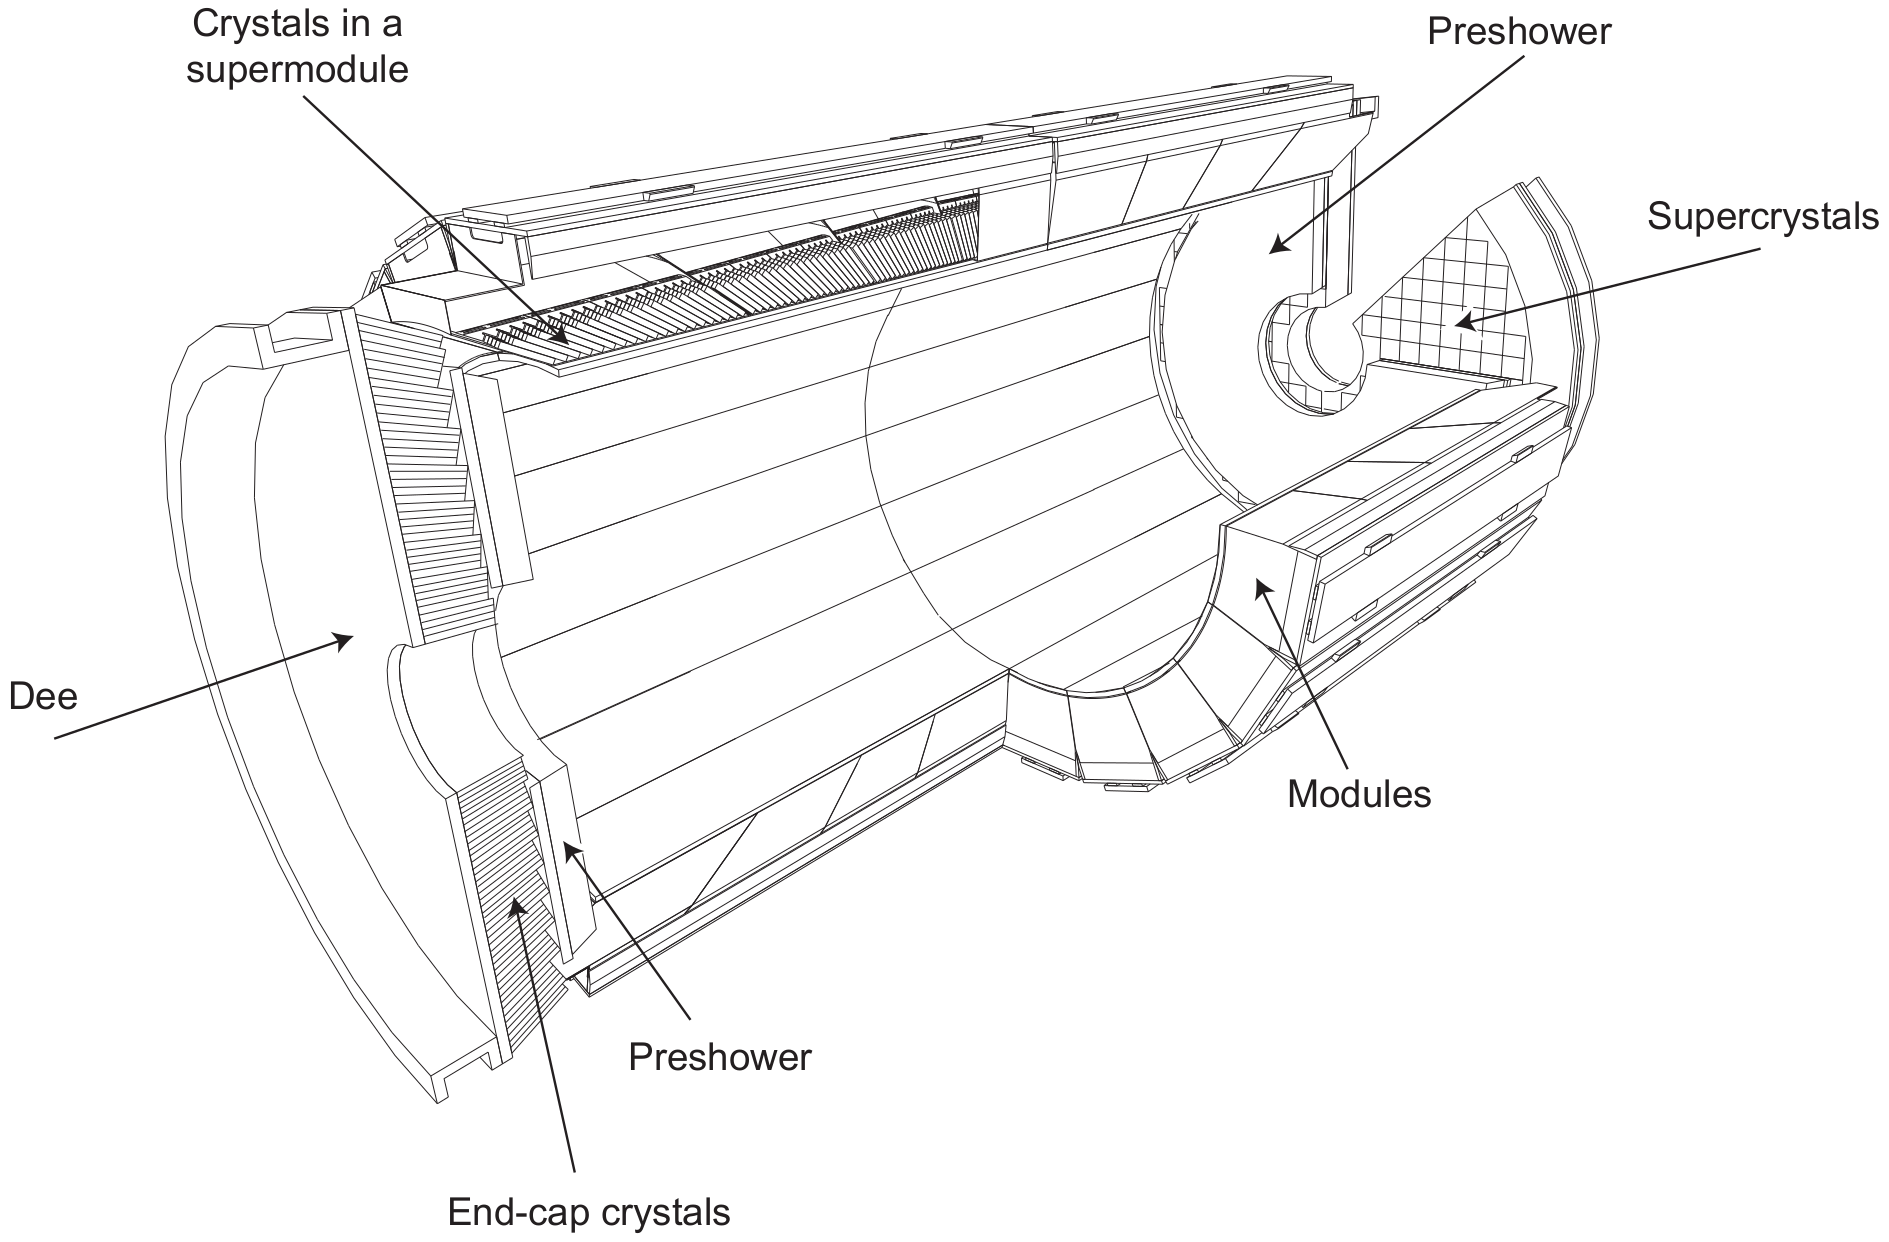
\includegraphics[width=0.9\textwidth]{\PhDthesisdir/plots_and_images/from_CMS-EGM-11-001/figures_calorimeter.png}
\caption[Schéma du calorimètre électronique de CMS.]{Schéma du calorimètre électronique de CMS~\cite{cms_paper,CMS-EGM-11-001} montrant le positionnement des cristaux, modules et supermodules dans le \CMSbarrel, des supercristaux et du détecteur de gerbes dans les \CMSendcaps.}
\label{fig-chapter-LHC-section-CMS-subsec-ECAL-CMS-EGM-11-001-figures_calorimeter}
\end{figure}
\par Le ECAL se divise en trois sous-parties, schématisées sur la figure~\ref{fig-chapter-LHC-section-CMS-subsec-ECAL-CMS-EGM-11-001-figures_calorimeter}.
Le \CMSbarrel\ du ECAL (EB) couvre la région $\abs{\eta}<\num{1.479}$.
La face frontale des cristaux du EB se trouvent à \SI{1.29}{\meter} du faisceau.
%Ils sont regroupés en \og modules \fg{} de \num{400} à \num{500} cristaux et quatre de ces modules forment un \og supermodule \fg{} de \num{1700} cristaux.
%Le tour complet du \CMSbarrel\ comporte \num{18} supermodules, chacun couvrant \ang{20} en $\phi$ et la moitié de l'espace en $\eta$ du EB.
%Le EB complet est ainsi formé de \num{36} supermodules.
%\par
Les \CMSendcaps\ du ECAL (EE) couvrent la région $\num{1.479}<\abs{\eta}<\num{3.0}$ et se trouvent à \SI{315.4}{\centi\meter} du point de collision le long de l'axe du faisceau.
%Cette distance prend en compte le mouvement de \SI{1.6}{\centi\meter} de cette partie du détecteur lorsque le champ magnétique de \SI{3.8}{\tesla} est présent.
%Sur deux demi-disques (\emph{dee}) par \CMSendcap\ sont répartis des \og supercristaux \fg{} formés de $5\times5$ cristaux.
\par Devant les EE se trouvent les détecteurs de gerbes (\emph{PreShower}).
Leur rôle est d'identifier les pions neutres dans la région $\num{1.653}<\abs{\eta}<\num{2.6}$.
Ces particules se propagent sur des distances moyennes de \SI{26}{\nano\meter} puis se désintègrent dans \SI{99}{\%} des cas en deux photons~\cite{PDG_booklet_2020}.
Ce sont donc ces deux photons que le \emph{PreShower} doit identifier.
Ce dernier aide à discriminer les électrons vis-à-vis des particules ionisantes ainsi qu'à la détermination des positions des photons et électrons.
Il est composé d'une couche de plomb initiant la gerbe électromagnétique suivie d'un détecteur à pistes de silicium mesurant les dépôts d'énergie.
\par L'oxyde de tungstate de plomb est très dense, \SI{8.29}{\gram.\centi\meter^{-3}}, et transparent.
Ce matériau possède également une faible longueur d'interaction, $X_0=\SI{0.89}{\centi\meter}$, ainsi qu'un rayon de Molière de \SI{2.19}{\centi\meter}.
Le ECAL présente une réponse rapide, une bonne granularité et une résistance suffisante aux radiations.
Près de \SI{80}{\%} du signal lumineux émis dans les cristaux du ECAL par les électrons et photons se trouve en effet dans une fenêtre temporelle de \SI{25}{\nano\second}, la durée entre deux événements successifs au LHC~\cite{cms_paper}.
Dans le cas des hadrons, la traversée des cristaux du ECAL correspond approximativement à une longueur d'interaction.
Près des deux tiers des hadrons initient donc une gerbe hadronique dans le ECAL, \ie\ avant d'arriver dans le calorimètre hadronique.
\par Pour les électrons et les photons, la longueur des cristaux, \SI{23}{\centi\meter} dans le \CMSbarrel\ et \num{22} dans les \CMSendcaps, correspond respectivement à \num{25.8} et \num{24.7} longueurs d'interaction, permettant de d'absorber \SI{98}{\%} de leur énergie jusqu'à \SI{1}{\TeV}.
Ces particules ne se propagent donc pas, en bonne approximation, dans les parties suivantes du détecteur.
\par La réponse des cristaux du ECAL est contrôlée régulièrement par l'injection de signaux lumineux issus de lasers~\cite{CMS-DP-2019-005}.
La figure~\ref{fig-chapter-LHC-section-CMS-subsec-ECAL-CMS-DP-2019-005-histories_2011-2012-2015-2016-2017-2018_190208} présente l'évolution de la réponse des cristaux du ECAL depuis le début de l'exploitation du LHC.
La réponse se dégrade au cours du temps car les cristaux, bien que peu sensibles aux radiations, se trouvent dans un environnement à très fortes radiations.
Une perte de la transparence des cristaux est ainsi inévitable, diminuant leur réponse.
Des corrections sont alors appliquées afin d'assurer une stabilité temporelle de la réponse du ECAL.
De plus, la réponse des cristaux présente une forte dépendance thermique, de l'ordre de \SI{2}{\%/\degC}.
Un système de refroidissement assure une stabilité de la température des cristaux à $\pm\SI{0.5}{\degC}$.
\begin{figure}[h]
\centering
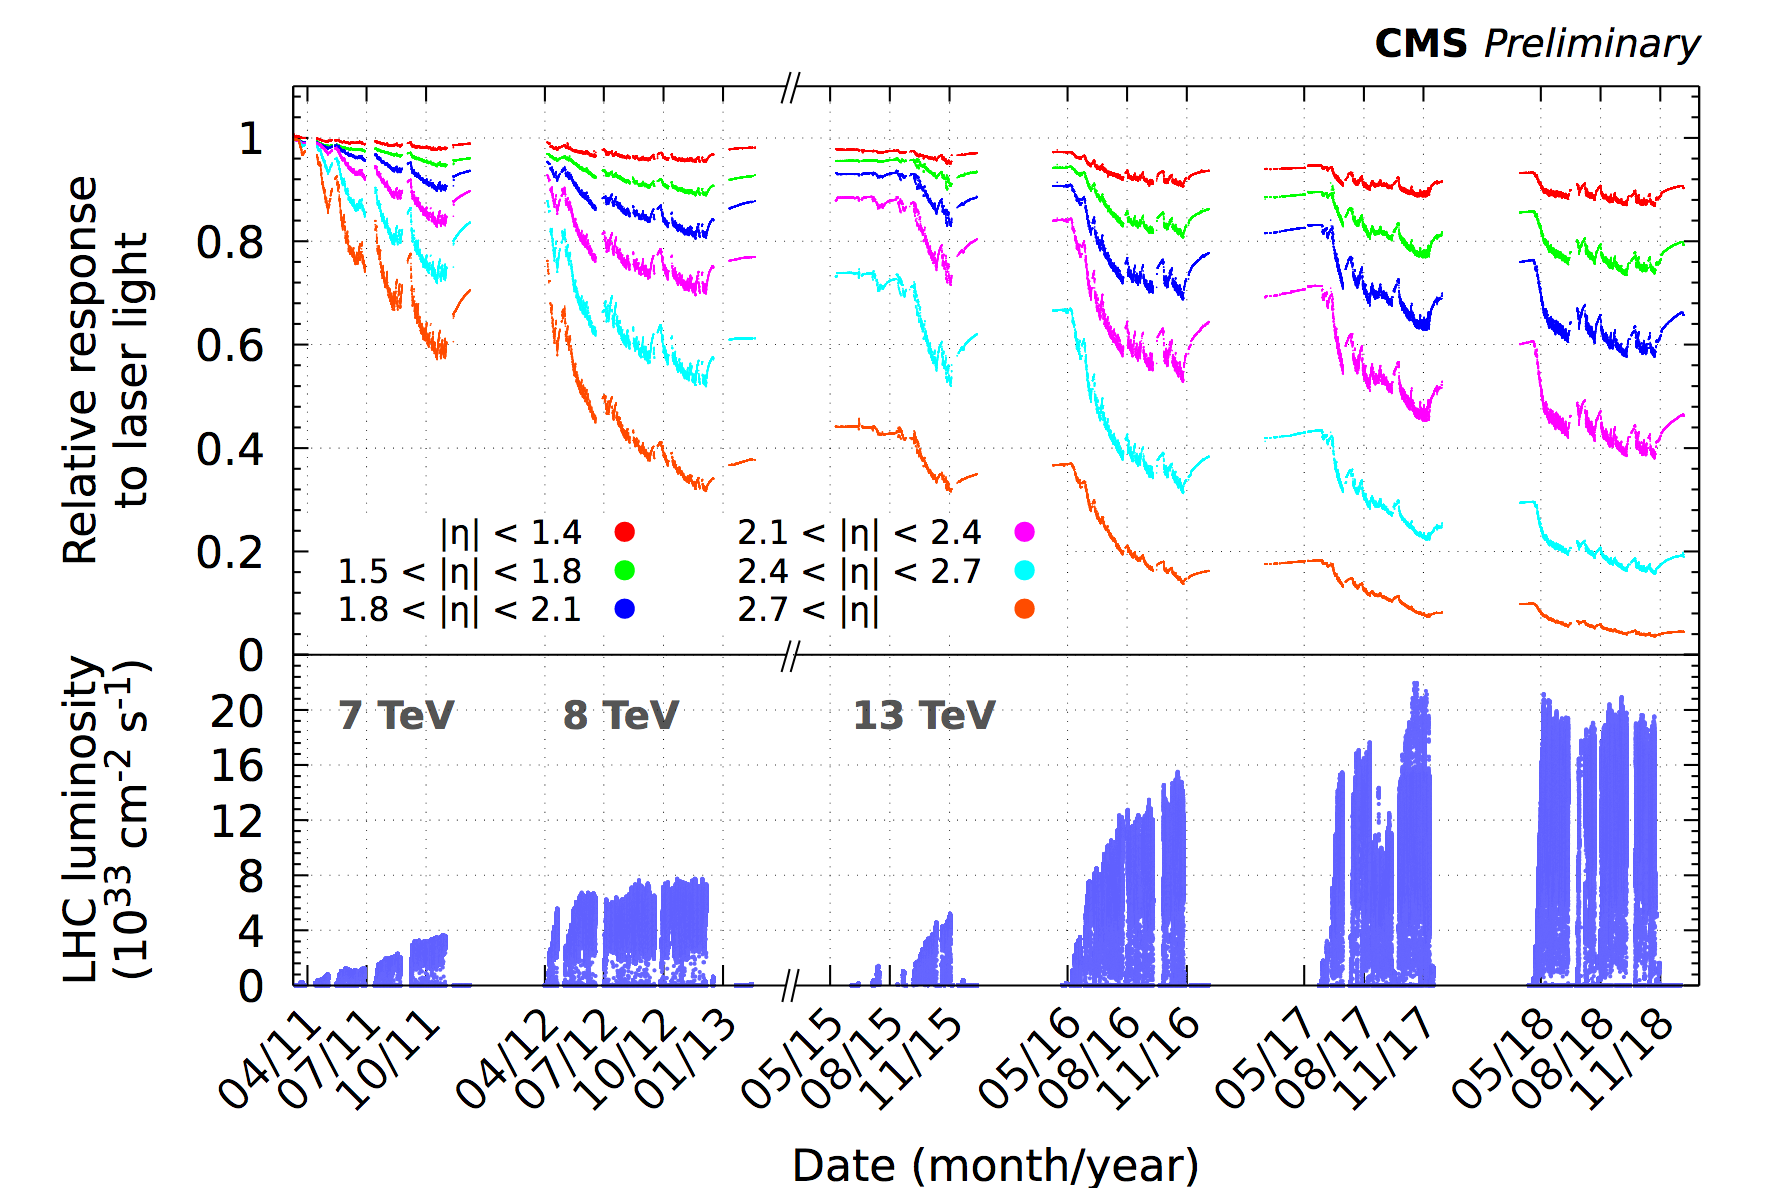
\includegraphics[width=.75\textwidth]{\PhDthesisdir/plots_and_images/from_CMS-DP-2019-005/histories_2011-2012-2015-2016-2017-2018_190208.png}
\caption[Évolution temporelle de la réponse du ECAL.]{Évolution temporelle de la réponse du ECAL~\cite{CMS-DP-2019-005} (haut) et luminosité instantanée du LHC (bas).}
\label{fig-chapter-LHC-section-CMS-subsec-ECAL-CMS-DP-2019-005-histories_2011-2012-2015-2016-2017-2018_190208}
\end{figure}
\par La résolution $\sigma$ du ECAL est paramétrée selon
\begin{equation}
\frac{\sigma}{E}
=
\frac{S}{\sqrt{E}}
\oplus
\frac{N}{E}
\oplus
C
\end{equation}
où $\oplus$ désigne une somme quadratique,
$S$ est un terme stochastique prenant en compte la largeur latérale de la gerbe électronique,
$N$ le terme de bruit des composants électroniques et
$C$ une constante rendant compte des erreurs de calibration.
Des tests en faisceau réalisés en 2006~\cite{cms_paper} ont permis de mesurer
$S = \SI{0.028}{\GeV^{1/2}}$,
$N = \SI{0.12}{\GeV}$ et
$C = \num{3.0e-3}$.
La figure~\ref{fig-chapter-LHC-section-CMS-subsec-ECAL-CMS-DP-2020-021-final_Resolution_RunII_Inclusive} présente la résolution relative du ECAL sur l'énergie des électrons lors du Run~II.
\begin{figure}[h]
\centering
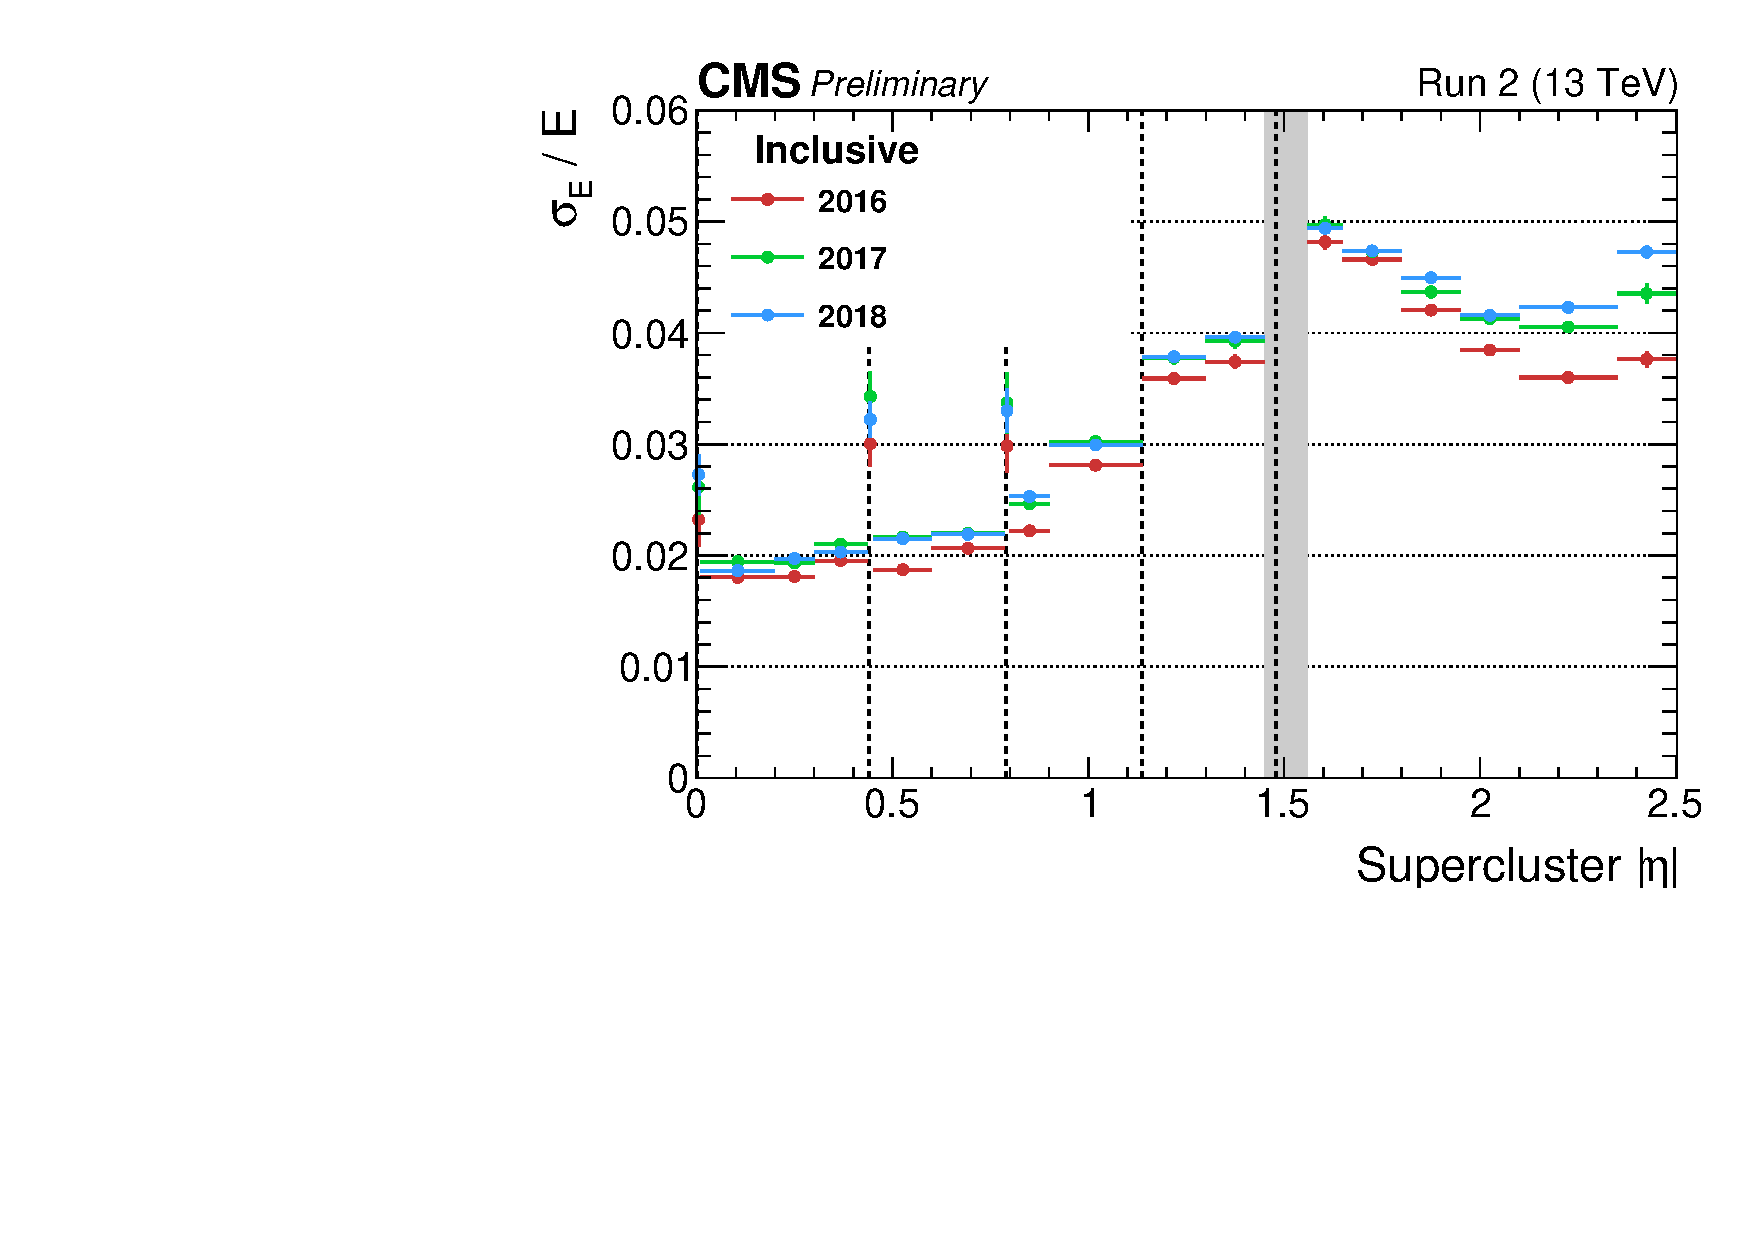
\includegraphics[width=.55\textwidth]{\PhDthesisdir/plots_and_images/from_CMS-DP-2020-021/final_Resolution_RunII_Inclusive.pdf}
\caption[Résolution relative de l'énergie des électrons dans le ECAL lors du Run~II.]{Résolution relative de l'énergie des électrons dans le ECAL lors du Run~II en fonction de $\eta$~\cite{CMS-DP-2020-021}. La résolution est obtenue à partir d'événements $\Zboson\to\antielectron\electron$.}
\label{fig-chapter-LHC-section-CMS-subsec-ECAL-CMS-DP-2020-021-final_Resolution_RunII_Inclusive}
\end{figure}